% !TEX root = ../swputhesis.tex
\chapter{网络流量异常数据检测系统设计与实现}

\section{引言}
在前文的研究中，针对工业互联网及企业网络流量中普遍存在的长尾
分布与未知攻击威胁，本文分别在第三章提出了基于实例多样性加权
的无监督超球体学习方法（IED-Deep SVDD），以及在第四章构建
了面向未知攻击的多模式无监督聚类检测框架。这两部分研究成果从
理论层面解决了单一模型难以覆盖稀疏正常样本以及难以刻画复杂多
模态流量分布的难题，为网络流量异常检测提供了坚实的算法基础。

然而，仅有理论模型与离线实验验证并不足以满足实际网络安全运维
的需求。在真实的网络环境中，异常检测不仅要求算法具备高准确率
与鲁棒性，还要求系统能够实时采集流量数据、快速响应检测请求、
直观展示检测结果并提供可视化的分析界面。为了验证本文所提算法
在实际应用场景中的有效性与工程可行性，有必要将其集成到一个完
整的软件系统中，实现从数据接入、预处理、模型推理到告警展示的
全流程自动化。

基于此，本章将设计并实现一套网络流量异常数据检测系统。该系统以
第三章和第四章提出的核心算法为检测引擎，结合现代软件工程设计模
式，构建一个功能完善、交互友好的异常检测平台。本章首先对系统进
行详细的需求分析，明确系统的业务流程与功能指标；随后阐述系统的
总体架构设计与关键功能模块的实现细节；最后通过系统界面展示与功
能测试，对系统的可用性与检测性能进行综合评估。通过本章的系统实
现，旨在将理论研究转化为可落地的工程实践，进一步验证本文所提方
法在实际网络安全防护中的应用价值。

\section{需求分析}
网络流量异常数据检测系统的设计旨在构建一个集成化、可视化的流量
分析平台，通过模块化的软件工程设计满足不同网络环境下的安全运维
需求。本节主要从功能需求和非功能需求两个维度对系统进行详细阐述。

\subsection{系统功能需求}

根据系统总体设计的业务流程，本系统主要包含数据采集与预处理、模
型管理与训练、实时检测与告警、以及可视化分析与展示四大核心功能模块。

\textbf{数据采集与预处理功能}是整个系统的基础。系统首先需要具备多源
数据接入能力，既要支持用户上传标准的PCAP流量包文件或CSV格式的流量日志
文件进行离线分析，也要能够直接绑定服务器网卡接口，实时捕获进出网络的原
始数据包。在数据接入后，系统需自动执行数据清洗与格式化操作，识别并剔除
缺失值、重复值及格式错误的脏数据，并提供统一的数据转换接口，将不同来源的
非结构化流量数据转化为符合算法输入的结构化特征向量，为后续的模型训练提供
高质量的数据支撑。

\textbf{模型管理与训练功能}允许用户对检测算法的生命周期进行全流程管理。
系统应提供可视化的参数配置面板，使用户能够自定义训练轮数（Epochs）、批次
大小（Batch Size）以及学习率等关键超参数，而无需修改底层代码。在模型训练
过程中，系统需实时通过进度条和折线图展示训练进度及损失值（Loss）的变化趋势
，使用户直观了解模型的收敛状态。此外，系统还应支持模型持久化功能，能够将训练
完成的模型权重文件保存至本地数据库，并支持一键加载历史最优模型用于后续的检测任务。

\textbf{实时检测与告警功能}是系统的核心业务逻辑。该功能负责调用已加载的检
测模型，对每一条流入的流量记录计算异常得分（Anomaly Score），以此量化其偏
离正常模式的程度。系统需内置智能阈值判定机制，支持手动设定阈值和基于统计学的
自动阈值推荐两种模式。当流量样本的异常得分超过设定阈值时，系统应立即将其判定
为异常，并自动记录异常发生的具体时间、源IP地址、目的IP地址、端口号及异常类型
，最终生成详细的告警日志供运维人员审查。

\textbf{可视化分析与展示功能}旨在提升系统的可解释性与用户体验。系统需构
建流量态势大屏，以仪表盘形式实时展示当前系统的整体运行状态，包括总流量数、异
常检出数及实时吞吐率。同时，为了直观地展示模型效果，系统应支持特征空间可视化
，利用降维算法将高维流量特征映射至二维平面，通过散点图清晰呈现正常样本与异常
样本的分布差异。此外，系统还需提供历史报表查询功能，允许用户根据时间段、IP地
址或异常类型检索历史检测记录，并导出检测报告。

\subsection{非功能需求}

除了上述业务功能外，系统在性能、稳定性和易用性方面还需满足特定的工程指标，以确
保在实际生产环境中的可用性。

首先，系统必须满足\textbf{实时性需求}。在在线检测模式下，系统应具备高效的数
据吞吐能力，单条流量的特征提取、模型推理与结果判定的总延迟应控制在毫秒级范围内
，确保检测过程不会造成网络拥塞或明显的业务滞后。

其次，系统需具备极高的\textbf{稳定性与鲁棒性}。系统应支持7x24小时不间断运行，
在面对突发的高并发流量冲击或异常格式数据输入时，能够保持核心服务的稳定，不发生进
程崩溃或内存溢出，并具备自动错误捕获与服务恢复机制。

最后，系统应注重\textbf{易用性与环境兼容性}。人机交互界面（GUI）的设计应布局
合理、操作逻辑清晰，使得非算法专业背景的安全运维人员也能通过简单的点击和配置完成
复杂的模型训练与检测任务。同时，系统后端应基于主流的软件架构开发，能够兼容标准的
Linux和Windows服务器环境，前端界面应适配主流Web浏览器，确保跨平台的访问体验。

\section{系统总体设计}

\subsection{系统总体架构}

本系统遵循软件工程的高内聚、低耦合设计原则，采用分层架构模式构建。
依据系统内部的数据流向与业务逻辑处理层级，整体架构自上而下划分为应用表现层、
业务逻辑层、分析检测层以及数据资源层，同时辅以权限控制与日志记录两大纵向支撑体系，以确保系统的安全性与可维护性。
系统总体功能架构如图 \ref{fig:system_arch} 所示。

\begin{figure}[htbp]
\centering
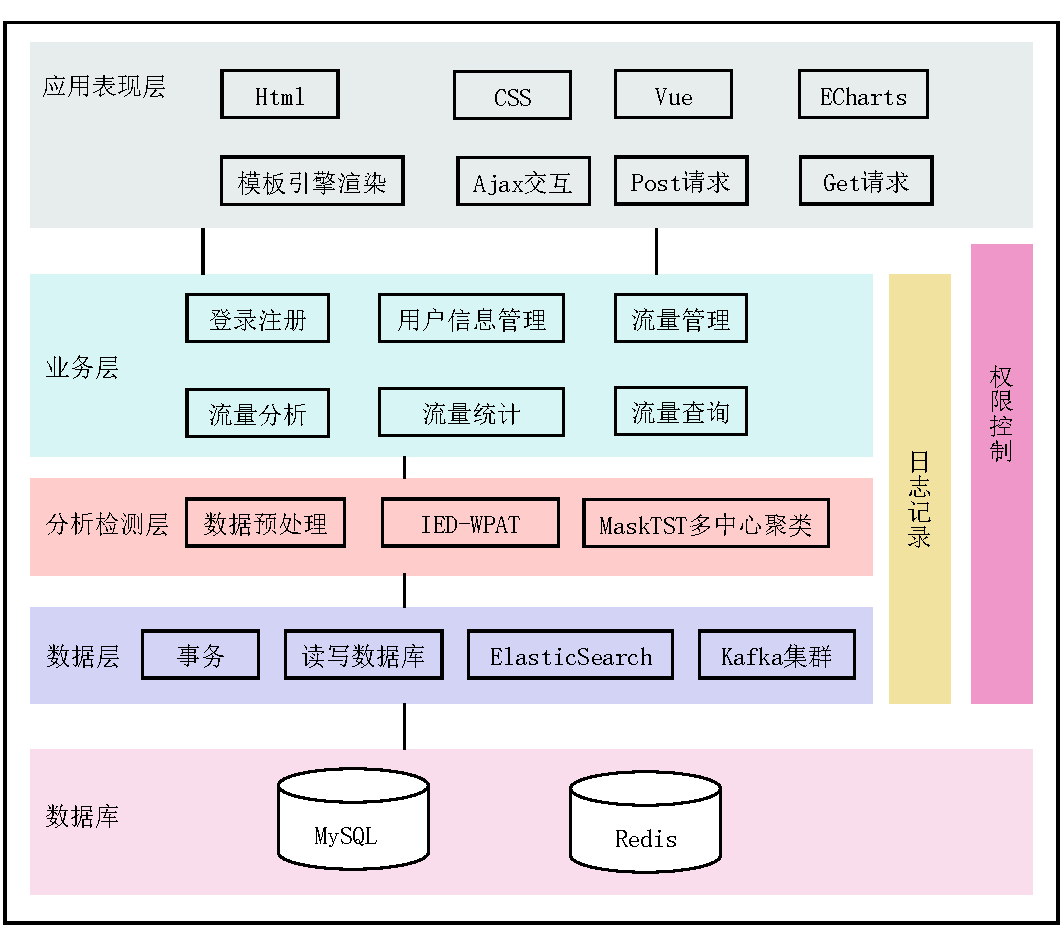
\includegraphics[width=0.95\linewidth]{fig/chapter5/第五章系统框架图.pdf}
\caption{基于流式处理的异常检测系统总体架构图}
\label{fig:system_arch}
\end{figure}

\subsection{应用表现与交互设计}

应用表现层位于架构最顶端，是用户与系统交互的直接窗口。
前端开发采用 Vue.js 组件化框架，结合 HTML5 与 CSS3 标准构建响应式用户界面。
为了直观展示复杂的网络流量数据，系统集成了 ECharts 可视化库，将抽象的流量特征转化为动态图表。
在交互模式上，系统摒弃了传统的整页刷新模式，采用 Ajax 异步通信技术。
前端通过构造标准化的 GET 或 POST 请求，与后端进行数据交换，经由模板引擎渲染后动态更新页面内容，
从而保证了操作的流畅性与即时性。

\subsection{业务逻辑层设计}

业务层是系统功能调度的核心枢纽，负责接收前端请求并协调底层资源。
该层包含五个关键功能模块：

\textbf{登录注册模块}负责用户的身份认证与会话管理；登录注册模块作为系统的安全准
入关口，集成了身份认证与会话管理的核心功能。前端基于 Vue.js 构建交互界面，对用户
输入进行格式预校验，并通过 Ajax 技术异步提交数据；后端服务采用加盐哈希算法对敏感凭
证进行加密处理与比对，同时引入 JWT (JSON Web Token) 令牌机制维持用户会话状态。
该模块通过严格的双重校验与加密传输机制，确保了用户身份的合法性，有效防止未授权访问，
为系统的业务安全提供基础保障。登录注册流程如图\ref{fig:login_register_flowchart}所示。
\begin{figure}[htbp]
	\centering
	
\includegraphics[scale=0.05]{fig/chapter5/登录注册功能流程图.png}
	\caption{登录注册模块流程图}
	\label{fig:login_register_flowchart}
\end{figure}

\textbf{用户信息管理模块}维护管理员与普通用户的资料及权限配置；用户信息管理模块是
系统权限管控与运维维护的基础单元，赋予管理员对系统用户数据的完整增删改查权限。 该模块
采用标准的前后端分离交互模式：前端 Vue.js 界面负责数据的展示与表单格式的实时预校验；
后端基于 FastAPI 接收 RESTful 请求，执行账号唯一性检查与业务逻辑验证。 所有数据变
更最终通过事务机制在 MySQL 数据库中原子生效，确保了用户配置数据的一致性与安全性，为
系统的分级授权管理提供了可靠支撑。用户信息管理模块的工作流程如图\ref{fig:user_info_flowchart}所示。
\begin{figure}[htbp]
	\centering
	\includegraphics[scale=0.05]{fig/chapter5/用户信息管理模块.png}
	\caption{用户信息管理模块流程图}
	\label{fig:user_info_flowchart}
\end{figure}

\textbf{流量分析模块}与\textbf{流量统计模块}流量分析与统计模块是系统的核心
计算引擎，实现了从微观流量检测到宏观态势感知的跨越。在实时分析侧，模块通过消费者线程
持续从 Kafka 拉取流量，经由数据预处理与 IED-Deep SVDD 模型并行推理，计算流量样本
与正常超球体的距离，实时判定异常等级并入库 Elasticsearch。在统计展示侧，后端基于 
FastAPI 提供聚合查询接口，利用倒排索引技术快速生成攻击趋势、高危 IP 排名及异常分布
热力图，为前端大屏提供毫秒级的数据可视化支撑，辅助运维人员精准研判网络安全态势。
流量分析与统计模块的工作流程如图\ref{fig:traffic_flowchart}所示。
\begin{figure}[htbp]
	\centering
	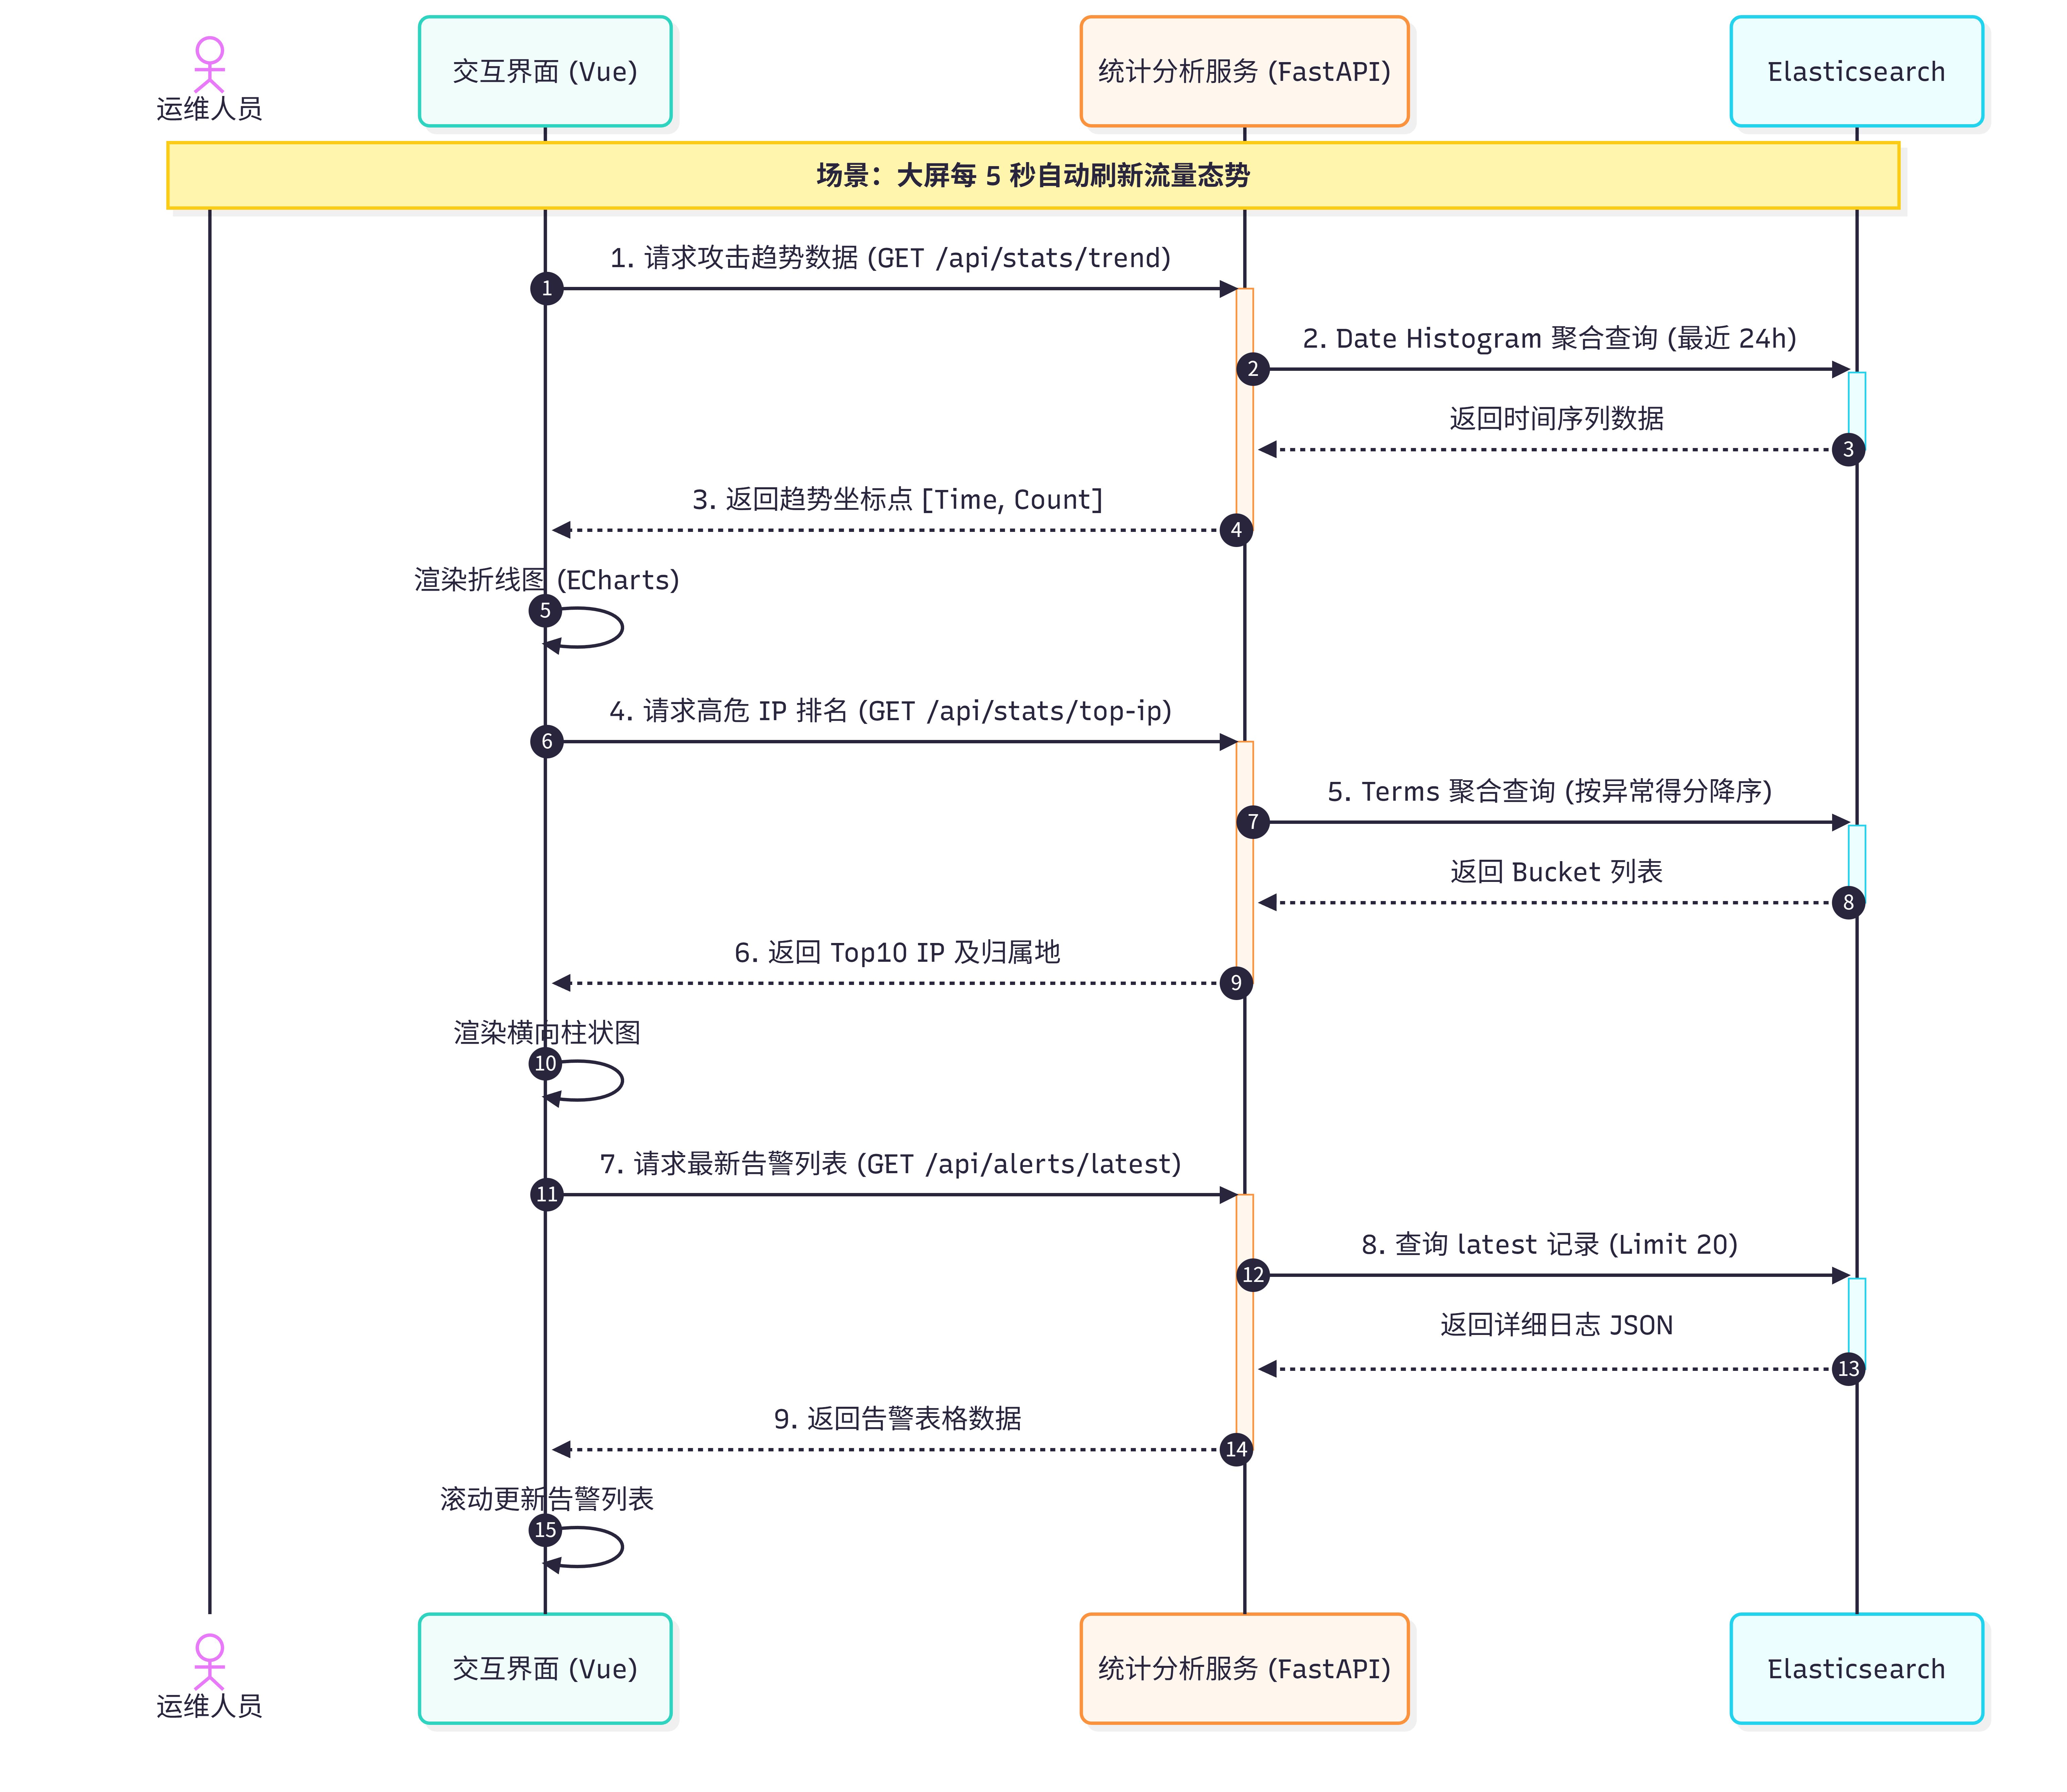
\includegraphics[scale=0.07]{fig/chapter5/流量分析与统计模块.png}
	\caption{流量分析与统计模块流程图}
	\label{fig:traffic_flowchart}
\end{figure}


\subsection{分析检测层设计}

分析检测层作为系统的“智慧大脑“，承载了本研究提出的双流并行检测架构。
数据进入该层后，首先触发\textbf{数据预处理}流水线，对多维流量特征向
量执行 Z-Score 标准化与 PCA 降维，消除量纲差异并降低计算复杂度，以适
配模型的输入空间。随后，预处理后的数据流被分发至并行部署的深度学习推理引擎
中：一方面，\textbf{IED-Deep SVDD 模型}将高维特征映射至潜空间，通过计算样
本到超球体中心 $c$ 的欧氏距离，精准识别偏离正常分布的长尾异常流量；另一方面，
\textbf{多模式聚类模型}利用无监督学习机制，针对未知的攻击模式进行特征聚类，
弥补单中心模型的检测盲区。最终，该层通过加权融合策略计算全局异常得分，将判定结
果实时推送至业务层用于告警展，并同步序列化至 Elasticsearch 实现持久化存储。
分析检测层的工作流程如图\ref{fig:analysis_flowchart}所示。
\begin{figure}[htbp]
	\centering
	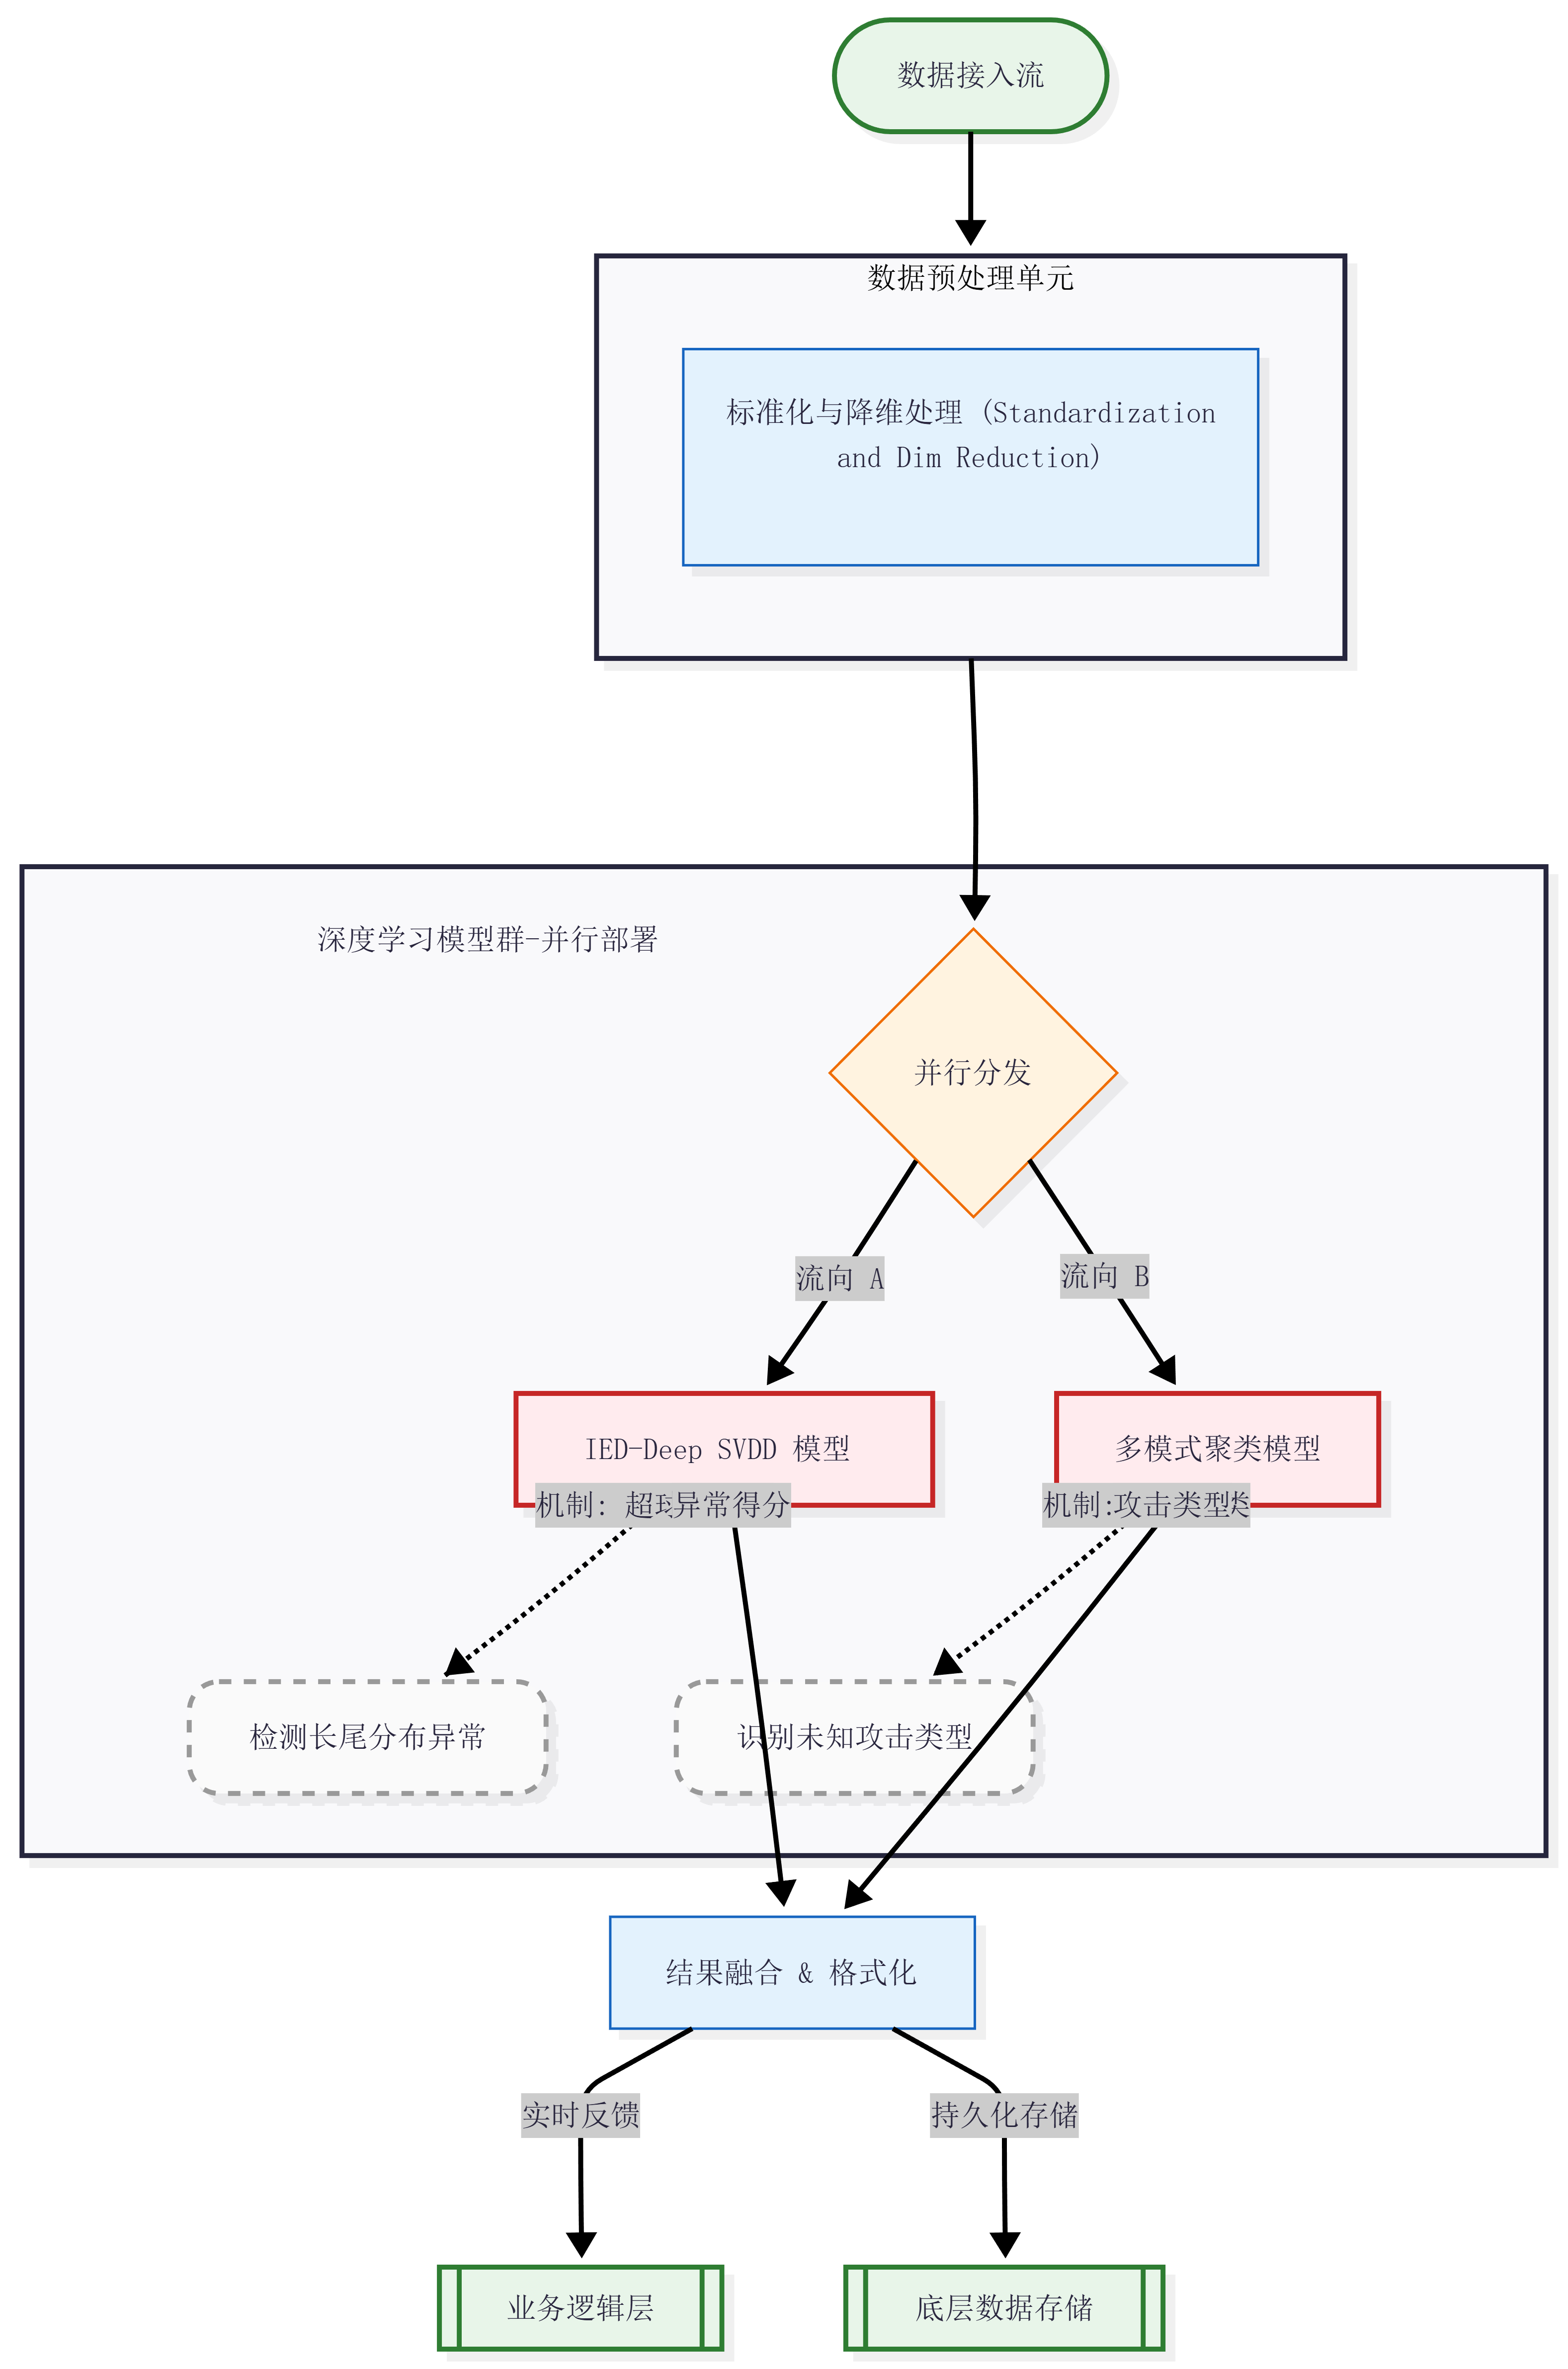
\includegraphics[scale=0.06]{fig/chapter5/分析检测层设计.png}
	\caption{分析检测层设计流程图}
	\label{fig:analysis_flowchart}
\end{figure}


\subsection{数据资源与存储设计}

数据层与数据库层构成了系统的基础设施底座，采用混合存储架构以应对不同类型的数据需求。
\textbf{数据层}集成了 Kafka 集群，作为高吞吐量的消息缓冲通道，实现流量数据的削峰填谷；
Elasticsearch 引擎用于海量日志的全文检索与快速分析。
\textbf{数据库层}则根据数据特性进行了异构选型：
选用 MySQL 关系型数据库存储用户信息、配置策略等结构化数据，确保事务的一致性；
同时引入 Redis 内存数据库作为缓存层，加速热点数据的读取，降低后端存储压力。
数据资源与存储设计工作流程如图\ref{fig:data_storage_flowchart}所示。

\subsection{跨层支撑体系}

为了保障系统的稳健运行，架构中设计了纵贯所有层级的支撑模块。
\textbf{权限控制体系}基于 RBAC（基于角色的访问控制）模型，
对应用层到数据层的每一次操作进行鉴权，防止越权访问。
\textbf{日志记录体系}则全方位监控系统运行状态，
记录用户操作日志与系统异常日志，为后续的故障排查与安全审计提供详实依据。

\begin{figure}[H]
	\centering
	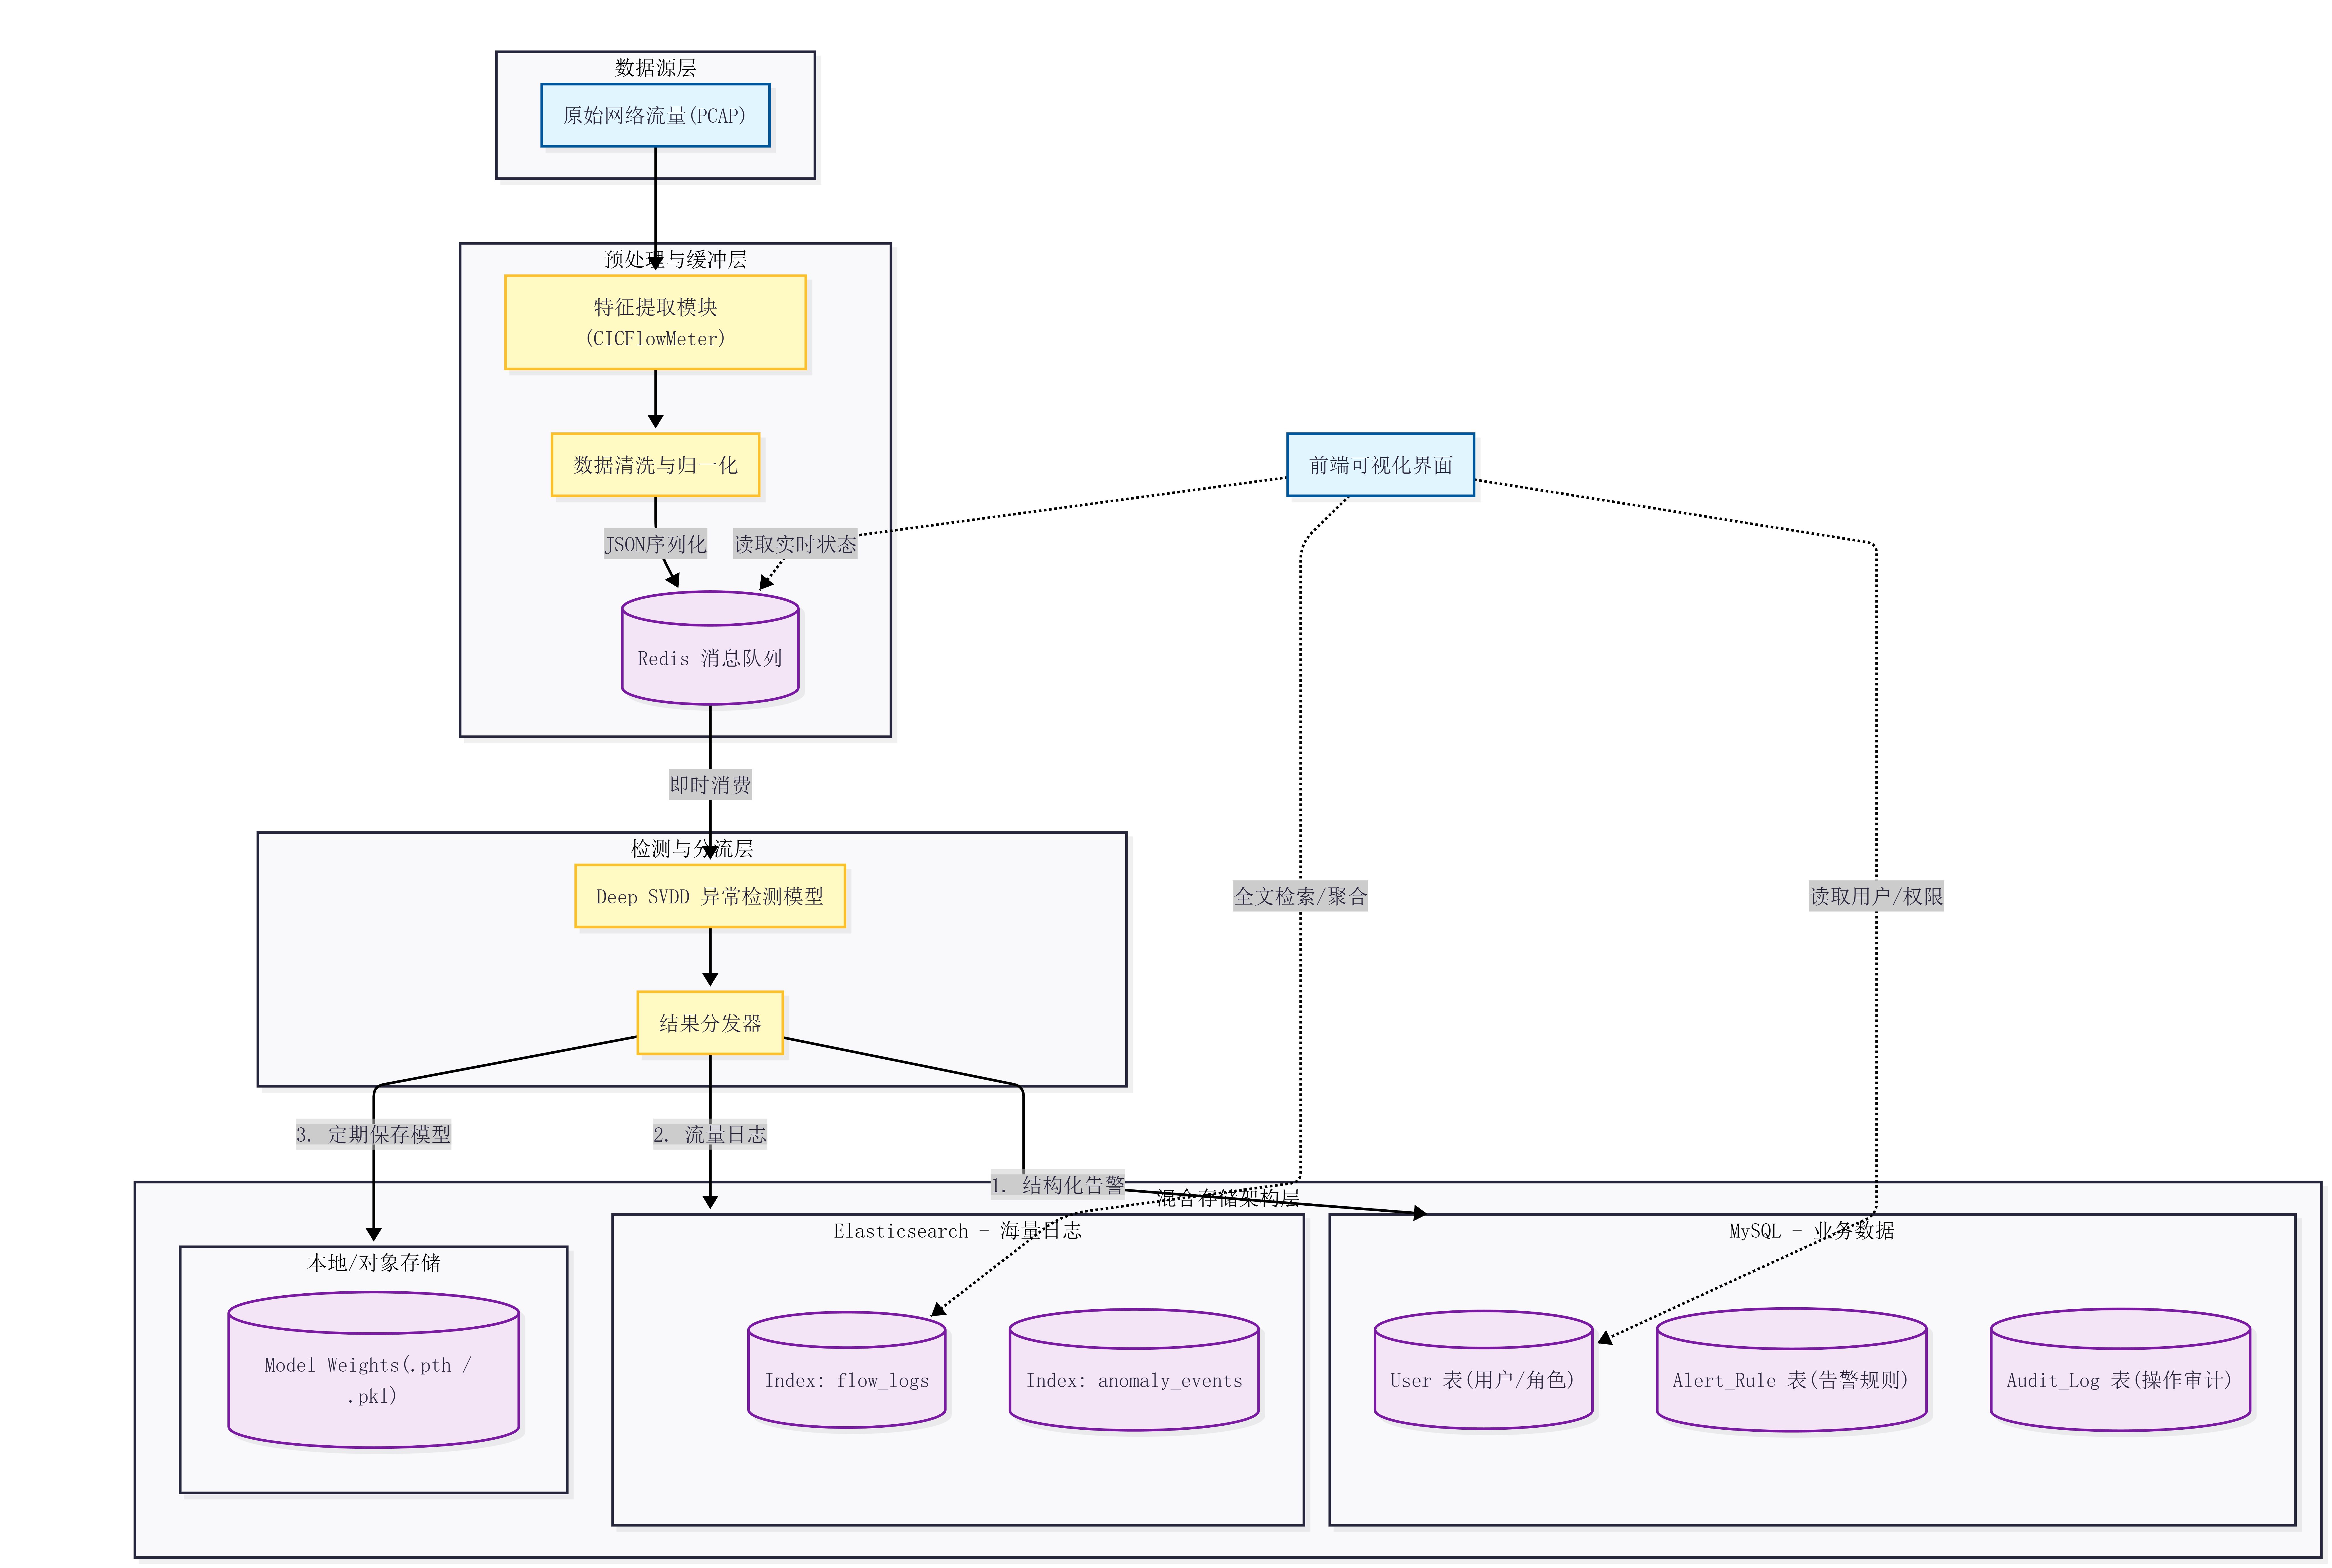
\includegraphics[scale=0.05]{fig/chapter5/数据资源与存储设计.png}
	\caption{数据资源与存储设计流程图}
	\label{fig:data_storage_flowchart}
\end{figure}

\section{系统界面展示}
基于前文的架构设计与核心功能模块实现，本节将对系统的实际运行界面进行展示。
前端基于 Vue.js 框架构建，采用 Element UI 组件库统一界面风格，并通过
 Axios 与后端 FastAPI 接口进行异步数据交互。以下按业务流程顺序，分别
 展示登录注册、态势感知大屏、流量分析详情及用户管理等核心界面。

\subsection{系统界面展示}

\textbf{1. 用户登录与注册界面}

登录界面是系统的安全准入关口。设计上采用极简风格，背景动态渲染粒子特效以
提升科技感。系统在此处集成了双重校验机制：前端利用正则表达式对邮箱格式与
密码强度进行实时检测，后端则校验账号的唯一性与凭证的合法性。注册流程与登
录流程无缝切换，用户注册成功后，系统会自动下发 JWT 令牌并跳转至主界面，
如图~\ref{fig:login_page}~所示。

\begin{figure}[htbp]
\centering
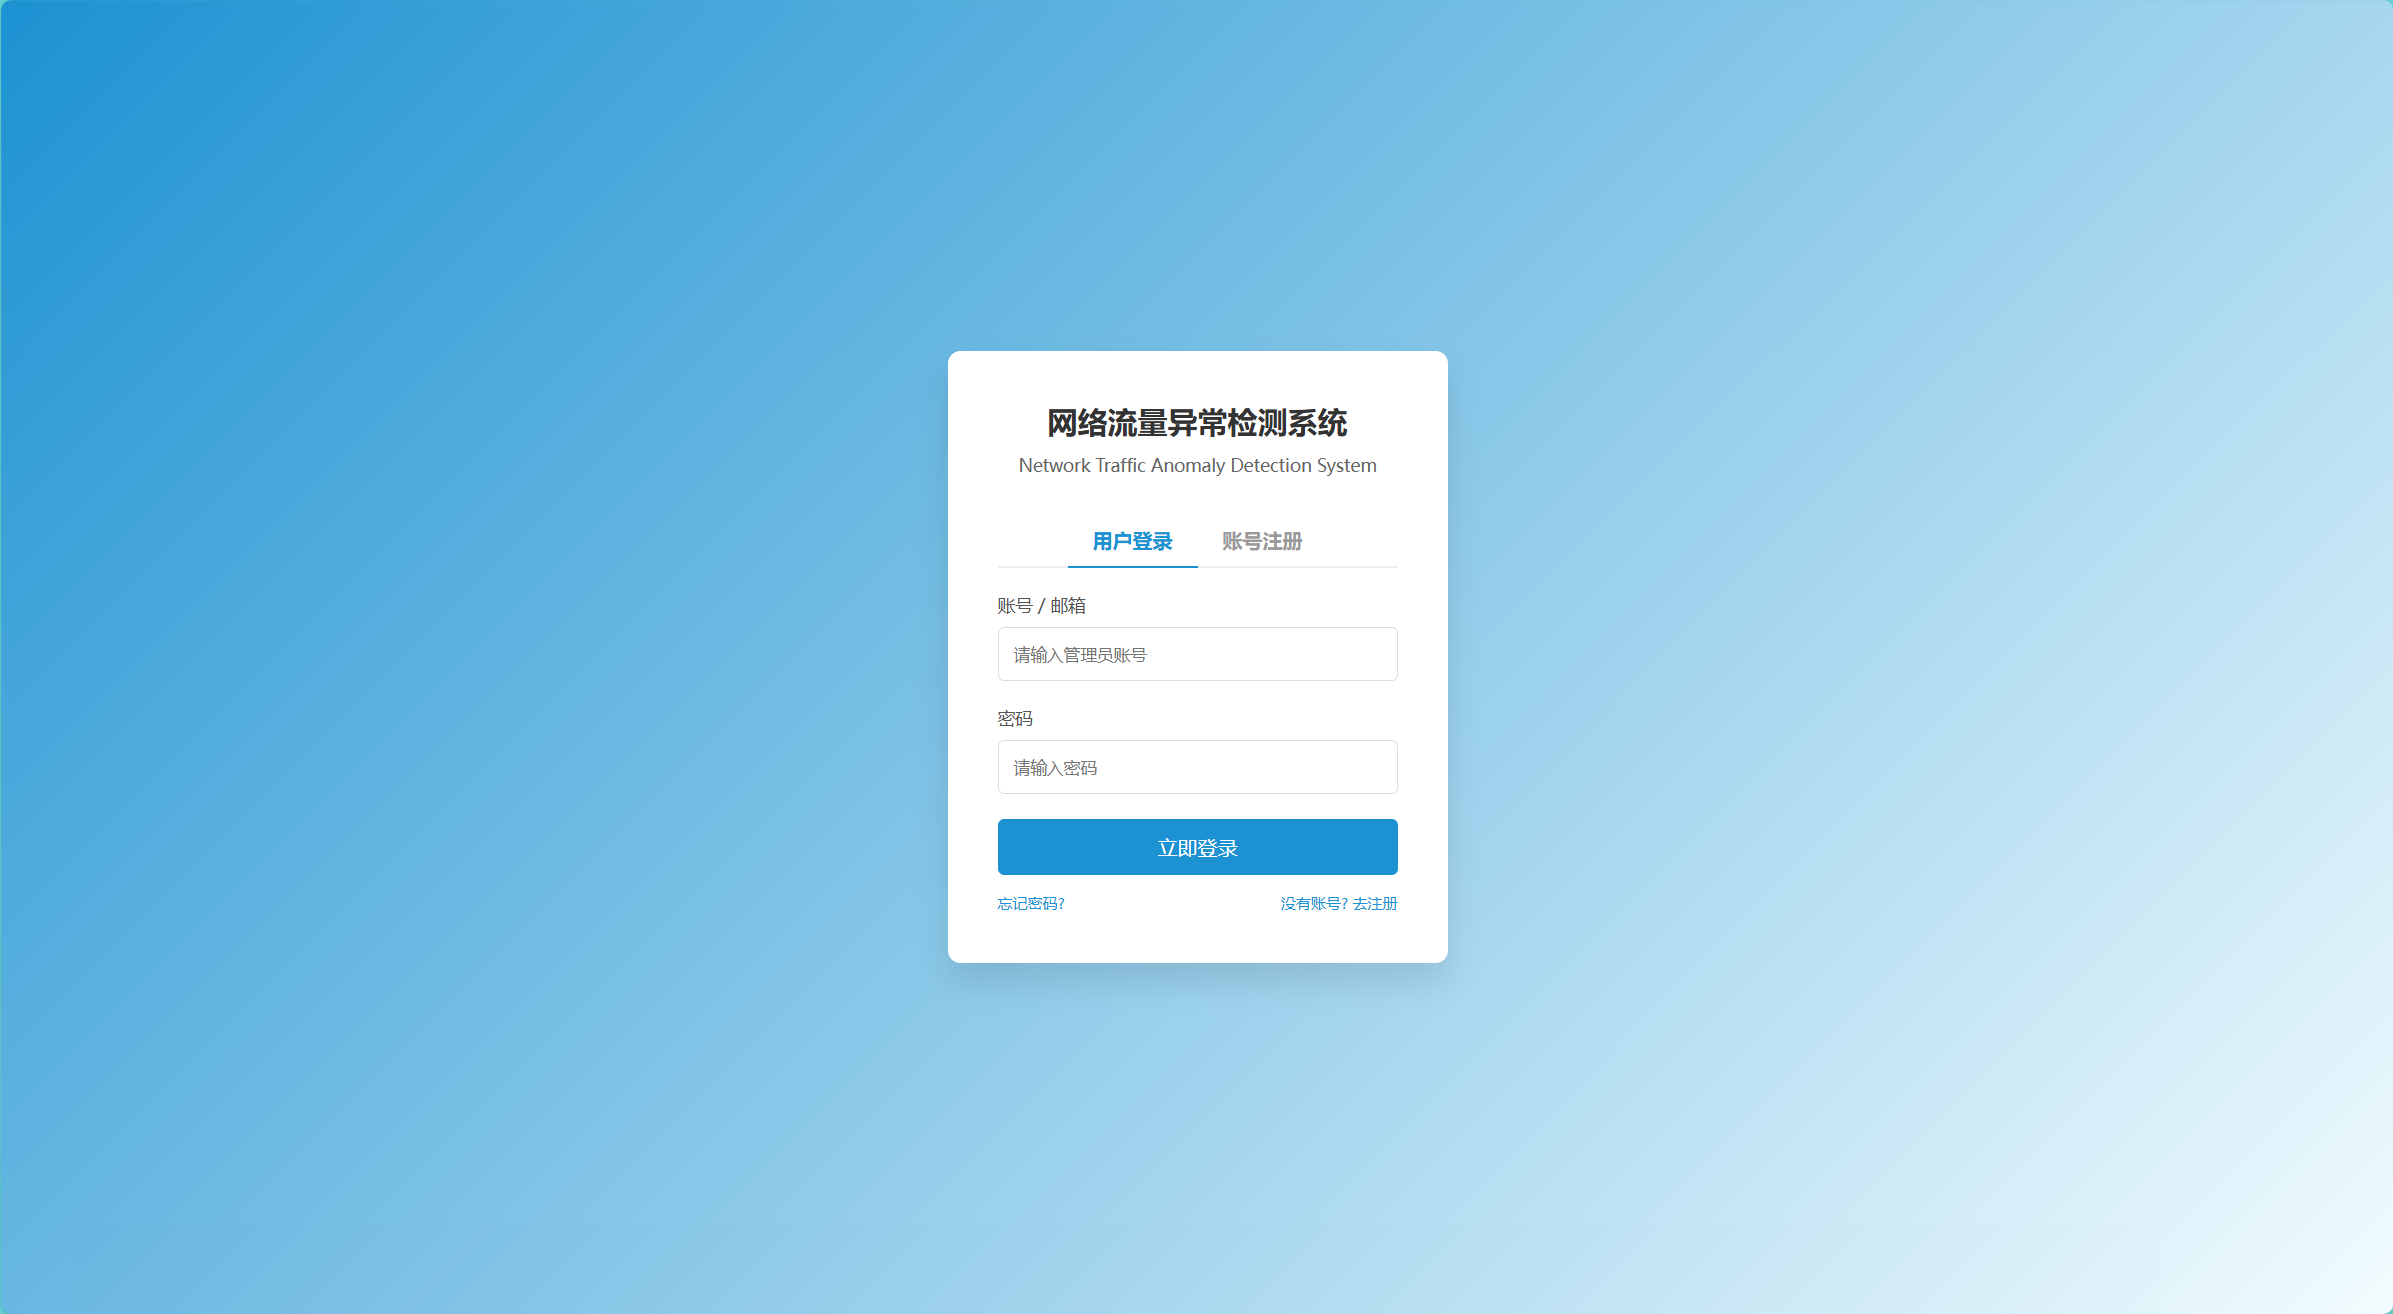
\includegraphics[width=0.8\linewidth]{fig/chapter5/login_interface.png}
\caption{系统用户登录与注册界面}
\label{fig:login_page}
\end{figure}

\textbf{2. 流量态势感知大屏}

态势感知大屏是本系统的可视化核心，旨在让运维人员“一屏览全局”。该界面集成 
ECharts 图表库，通过轮询接口实时从 Elasticsearch 拉取聚合数据。界面布
局分为三个区域：顶部展示当前系统的关键指标（如总流量、今日告警数、防御拦截
率）；中部左侧绘制“24 小时流量趋势折线图”，直观反映流量的波峰波谷；中部右
侧展示“攻击源 Top IP 排名”及“攻击类型分布饼图”。大屏界面如图~\ref{fig:dashboard}~所示，
能够帮助管理员快速定位高危目标。

\begin{figure}[htbp]
\centering
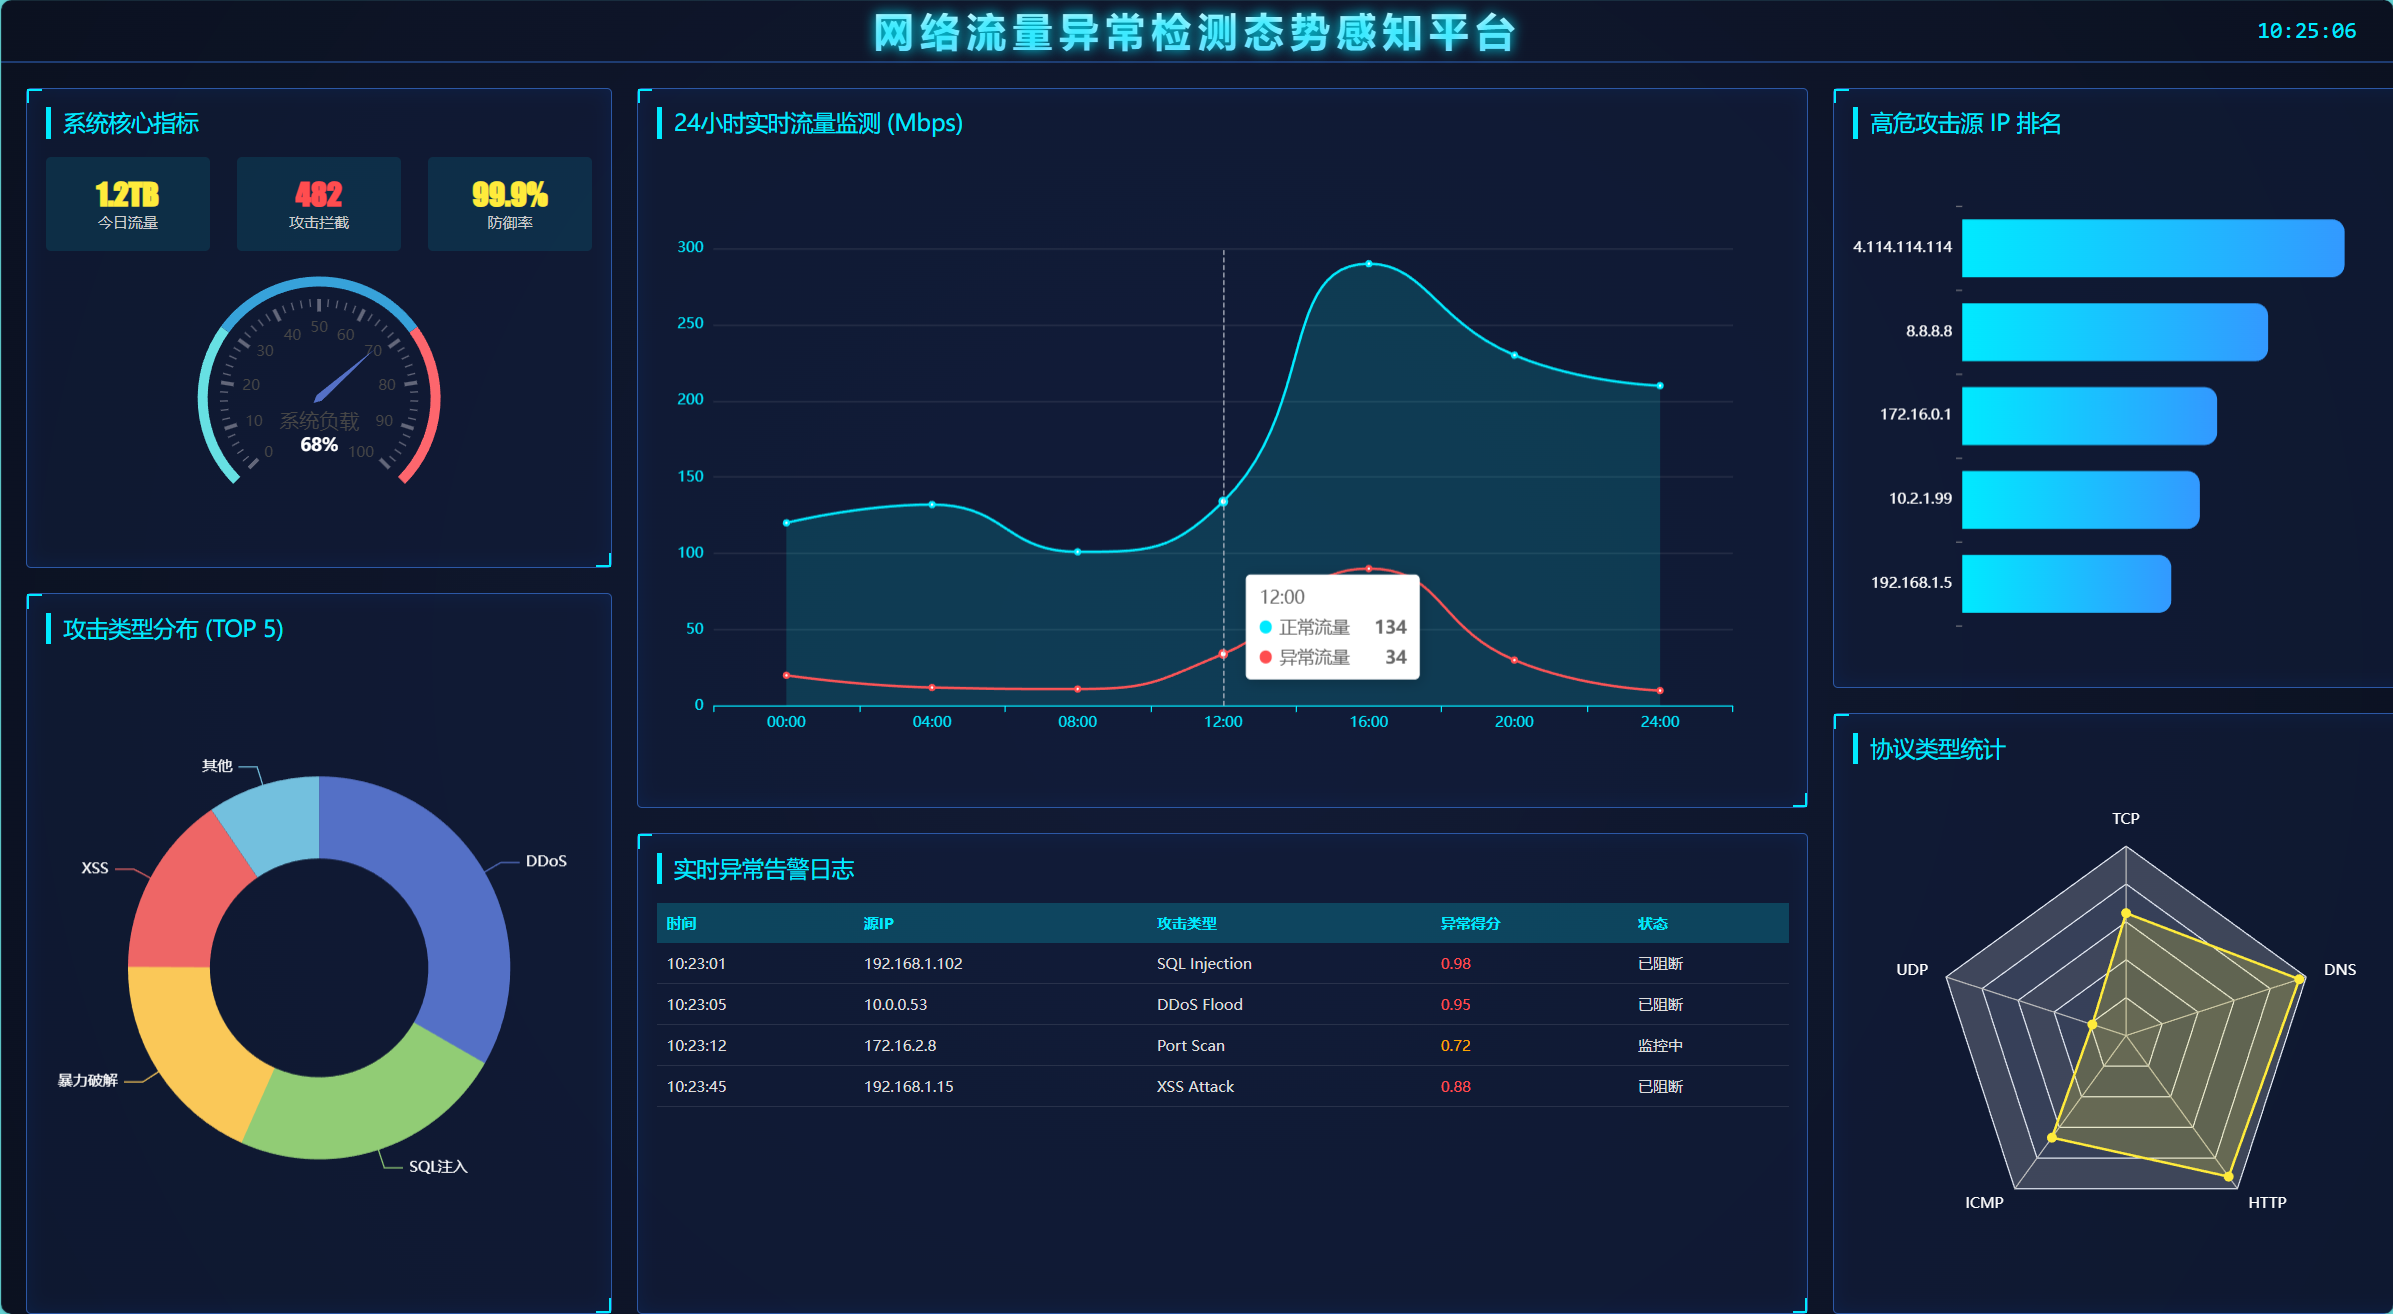
\includegraphics[width=0.8\linewidth]{fig/chapter5/dashboard_overview.png}
\caption{网络流量态势感知可视化大屏}
\label{fig:dashboard}
\end{figure}

\textbf{3. 异常流量分析详情页}

该界面主要用于展示分析检测层（Deep SVDD + 多模式聚类）的推理结果。界面主
体为一个可交互的数据表格，详细列出了每一条被判定为异常的流量记录，包含时间戳
、源/目的 IP、协议类型以及核心字段——\textbf{异常得分（Anomaly Score）}。
运维人员点击某条记录，可展开查看其五元组详情及所属的聚类簇信息。此外，界面上方配
有“异常得分分布散点图”，用红色标记超出超球体边界的离群点，直观验证了算法对长尾
流量的检测效果，如图~\ref{fig:traffic_analysis}~所示。

\begin{figure}[htbp]
\centering
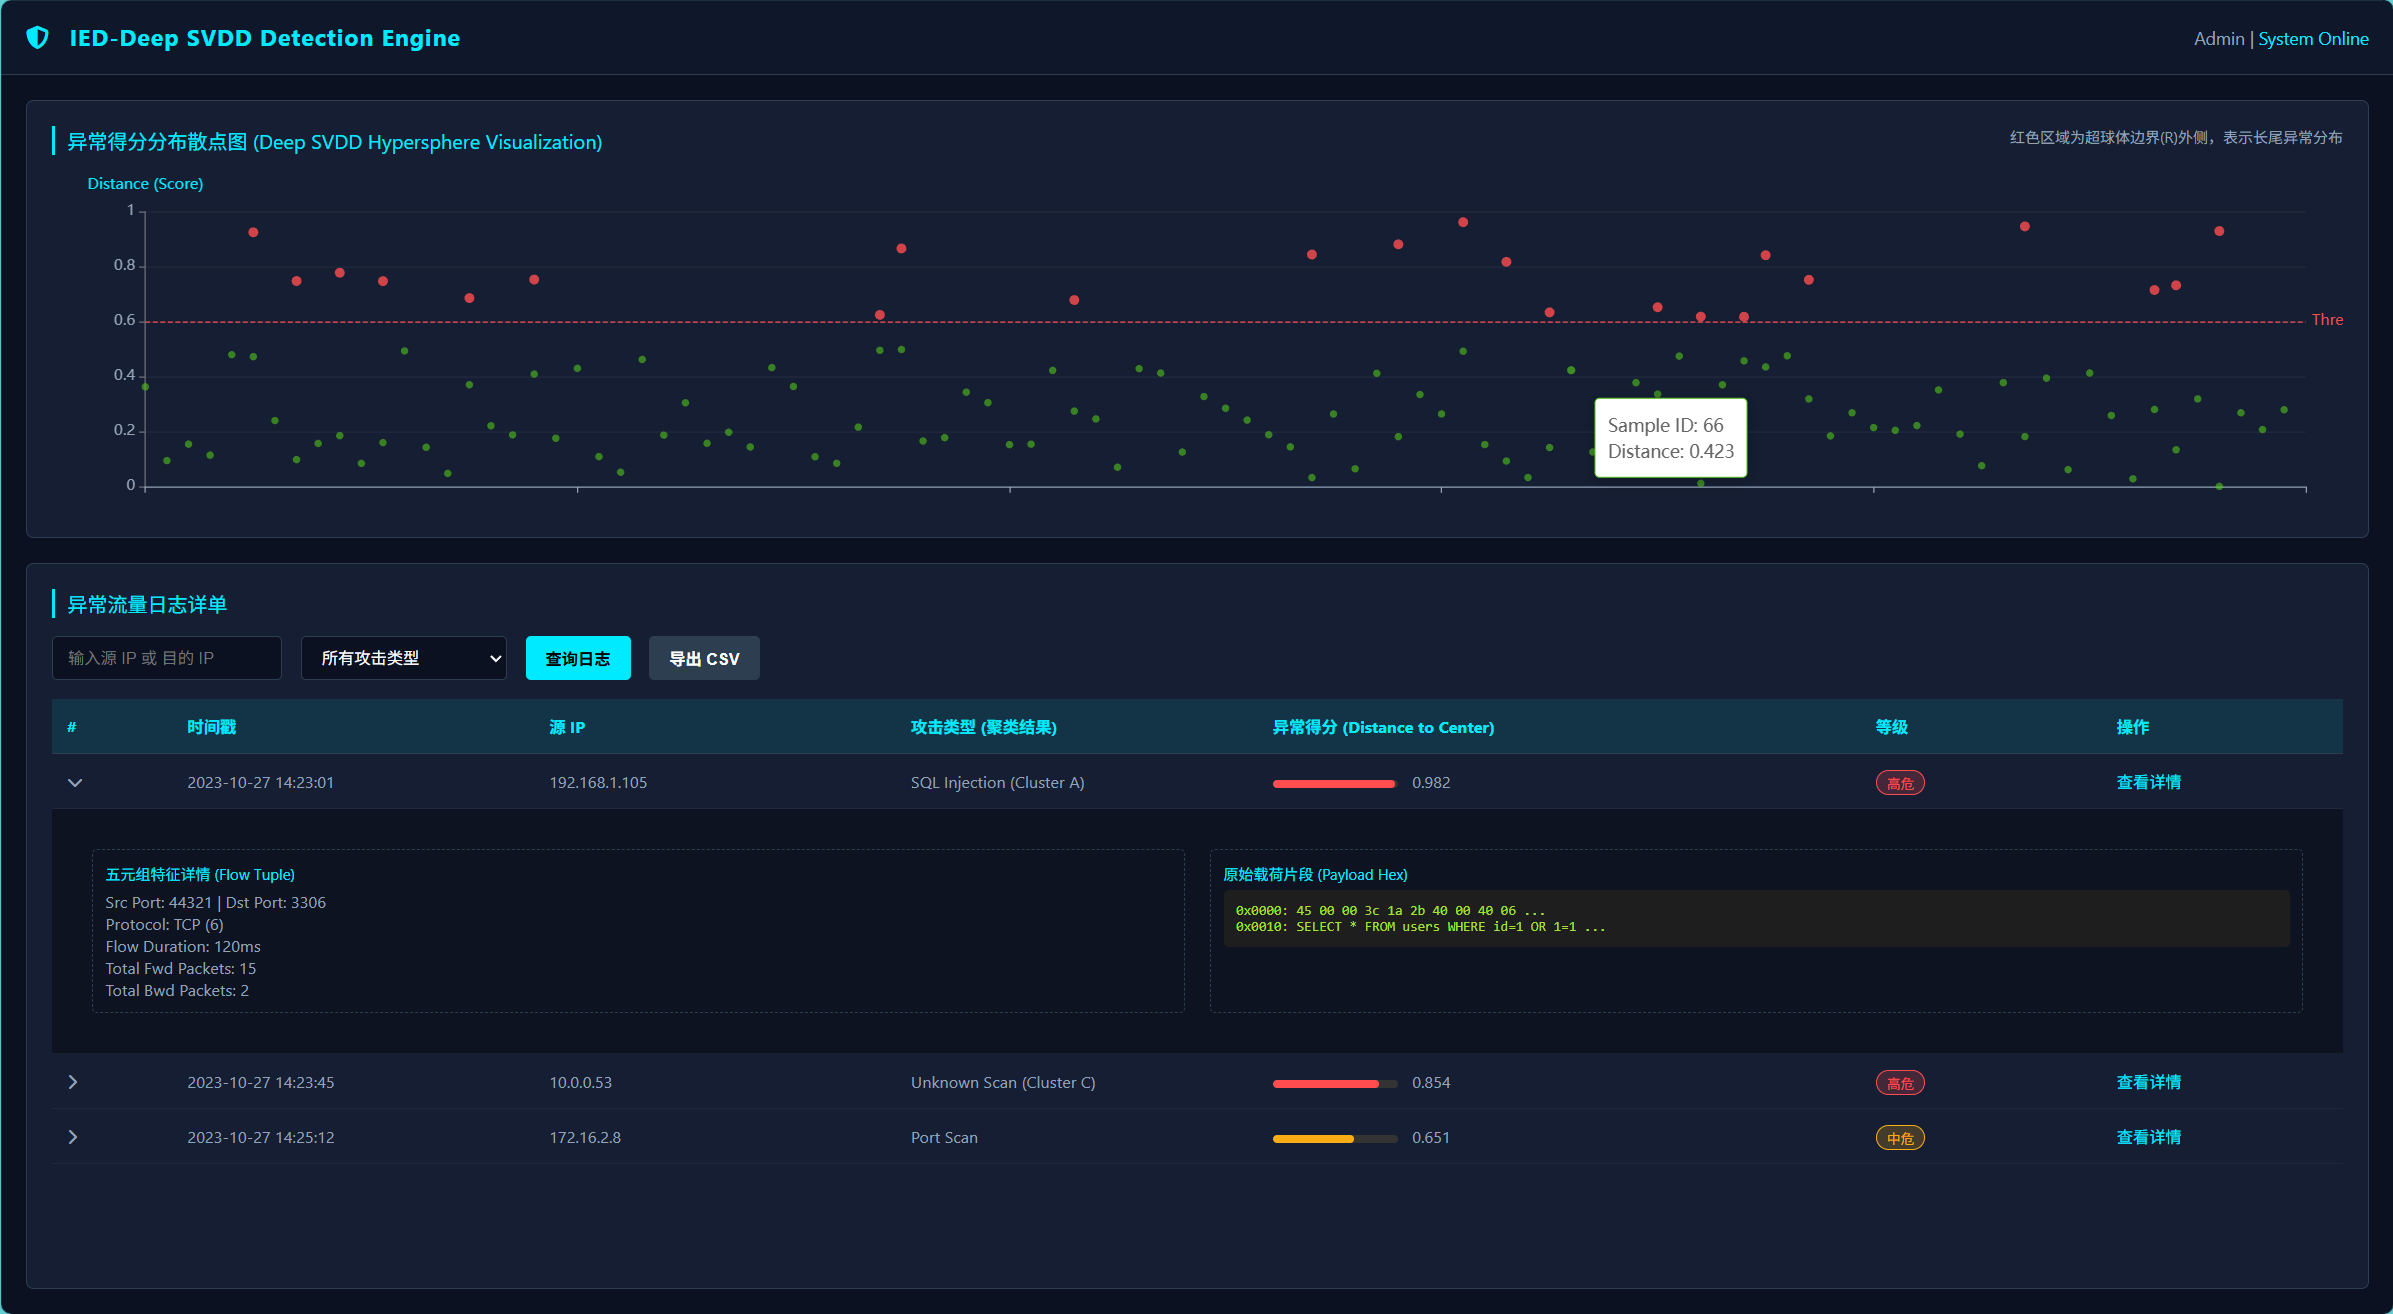
\includegraphics[width=0.8\linewidth]{fig/chapter5/traffic_analysis_detail.png}
\caption{异常流量检测结果详情界面}
\label{fig:traffic_analysis}
\end{figure}

\textbf{4. 系统用户管理界面}

该界面为管理员提供对系统用户的全生命周期管理能力。通过表格形式展示已注册用户信息，
支持按角色（管理员/普通用户）和状态进行筛选。操作栏提供了编辑与删除功能：点击“编辑”
会弹出模态框（Modal），回显当前用户信息供修改；点击“删除”则触发二次确认机制，防止误
操作。所有变更操作均通过 RESTful 接口同步至后端 MySQL 数据库，确保数据的一致性，
如图~\ref{fig:user_manage}~所示。

\begin{figure}[htbp]
\centering
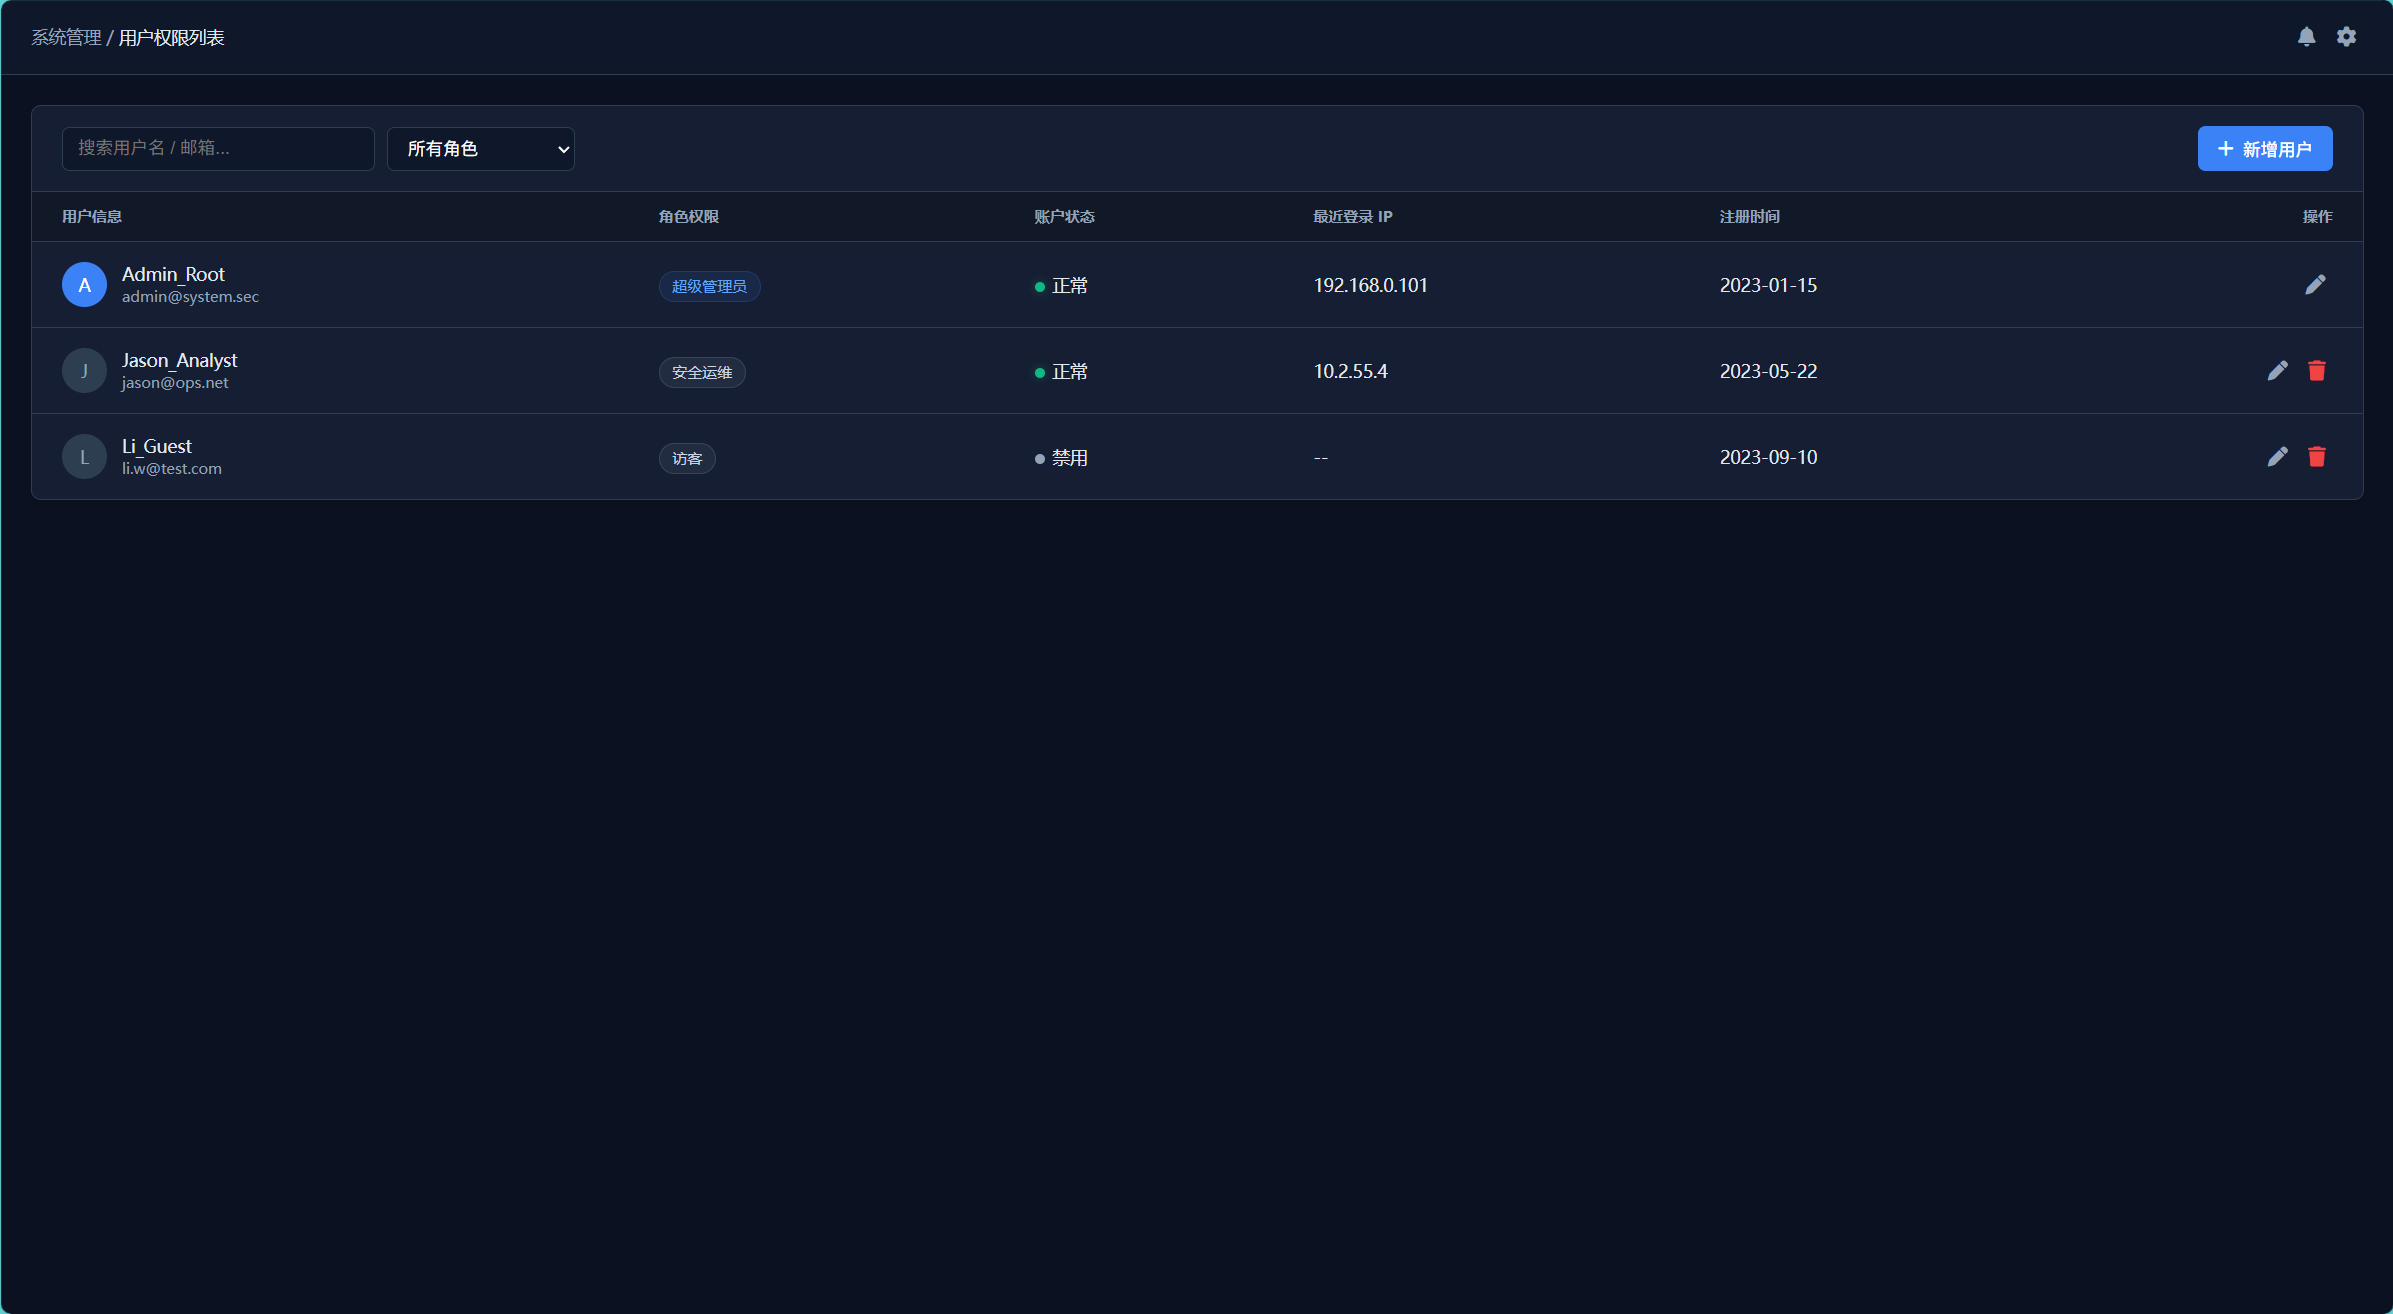
\includegraphics[width=0.9\linewidth]{fig/chapter5/user_management.png}
\caption{系统用户权限管理界面}
\label{fig:user_manage}
\end{figure}


\section{系统测试}
系统测试是软件开发生命周期中至关重要的一环，旨在验证系统是否满足需求分
析阶段确定的功能指标与性能指标。本节将从测试环境搭建、功能模块测试、性
能压力测试以及模型检测效果测试四个维度对网络流量异常检测系统进行全面的评估。

\subsection{测试环境配置}

为了确保测试结果的准确性与可复现性，本次测试在特定的软硬件环境下进行。
考虑到 Deep SVDD 模型对计算资源的需求，服务器端配置了高性能 GPU 
进行推理加速。
\begin{table}[htbp]
\centering
\caption{系统测试软硬件环境配置表}
\label{tab:5-3}
\begin{tabular}{p{2.5cm} p{3.5cm} p{6.5cm}}
\toprule
类别 & 项目 & 配置参数/版本说明 \\
\midrule
\multirow{4}{*}{硬件环境}
& 处理器 (CPU) & Intel Core i7-12700K @ 3.60GHz (12核) \\
& 内存 (RAM) & 32GB DDR4 3200MHz \\
& 显卡 (GPU) & NVIDIA GeForce RTX 3060 (12GB 显存) \\
& 存储 & 1TB NVMe SSD (用于高速存取流量日志) \\
\midrule
\multirow{4}{*}{软件环境}
& 操作系统 & Ubuntu 20.04 LTS (服务器端) / Windows 11 (客户端) \\
& 数据库 & MySQL 8.0, Redis 6.2, Elasticsearch 7.10 \\
& 开发语言/框架 & Python 3.9 (PyTorch 1.10), Vue 3.0 \\
\midrule
\multirow{3}{*}{测试工具}
& 接口测试 & Postman v9.0 \\
& 压力测试 & Apache JMeter 5.4 \\
& 流量回放 & TCPreplay / Wireshark \\
\bottomrule
\end{tabular}
\end{table}

\subsection{功能测试}

功能测试主要采用黑盒测试方法，依据第 3 章的需求分析，对系统的各个核心模块进行输入输出验证。

\textbf{1. 用户权限与登录模块测试}

测试目标：验证身份认证机制的安全性及权限控制的有效性。

\begin{table}[htbp]
\centering
\caption{用户权限与登录模块测试结果}
\begin{tabular}{p{1.5cm} p{3.5cm} p{2.5cm} p{3cm} p{3cm} p{1.5cm}}
\toprule
测试编号 & 测试用例描述 & 预置条件 & 输入数据 & 预期结果 & 测试结果 \\
\midrule
TC-01 & 用户正常登录 & 账号存在 & 正确的用户名与密码 & 跳转至系统首页，Token存入本地 & 通过 \\
TC-02 & 密码错误登录 & 账号存在 & 错误的密码 & 提示“账号或密码错误”，禁止进入 & 通过 \\
TC-03 & 越权访问测试 & 未登录状态 & 直接访问 /dashboard & 自动拦截并重定向至登录页 & 通过 \\
\bottomrule
\end{tabular}
\end{table}

\textbf{2. 流量实时监测与可视化模块测试}

测试目标：验证大屏数据展示的实时性与准确性。

\begin{table}[htbp]
\centering
\caption{流量实时监测与可视化模块测试结果}
\begin{tabular}{p{1.5cm} p{3.5cm} p{3cm} p{3.5cm} p{1.5cm}}
\toprule
测试编号 & 测试用例描述 & 操作步骤 & 预期结果 & 测试结果 \\
\midrule
TC-04 & 实时流量趋势图更新 & 启动后端数据流，观察大屏折线图 & 图表每 3 秒刷新一次，数据与日志一致 & 通过 \\
TC-05 & 异常告警日志展示 & 模拟发送 SQL 注入攻击流量 & 告警列表立即出现红色高亮条目 & 通过 \\
TC-06 & 攻击类型分布统计 & 模拟多种攻击流量 (DDoS, XSS) & 饼图能够正确统计各类型占比 & 通过 \\
\bottomrule
\end{tabular}
\end{table}

\textbf{3. 用户管理模块测试}

测试目标：验证管理员对系统用户的增删改查操作。

\begin{table}[htbp]
\centering
\caption{用户管理模块测试结果}
\begin{tabular}{p{1.5cm} p{3.5cm} p{3cm} p{3.5cm} p{1.5cm}}
\toprule
测试编号 & 测试用例描述 & 操作步骤 & 预期结果 & 测试结果 \\
\midrule
TC-07 & 新增用户 & 点击新增，填写完整信息并保存 & 列表刷新，新用户可成功登录 & 通过 \\
TC-08 & 删除用户 & 点击删除按钮，确认弹窗 & 用户从数据库移除，且无法登录 & 通过 \\
\bottomrule
\end{tabular}
\end{table}

\subsection{系统性能测试}

性能测试使用 Apache JMeter 模拟高并发网络流量请求，重点考察系统在流量高峰下
的响应时间 (Response Time) 和吞吐量 (Throughput)。

测试场景设置：模拟 500、1000、2000 个并发线程同时向检测接口发送流量特征数据。

持续时间：300 秒。

\begin{table}[htbp]
\centering
\caption{接口并发性能测试结果}
\label{tab:5-4}
\begin{tabular}{p{2cm} p{2.5cm} p{2.8cm} p{2.2cm} p{2cm} p{2cm}}
\toprule
并发数 (Users) & 平均响应时间 (ms) & 99\% 响应时间 (ms) & 吞吐量 (QPS) & 错误率 (\%) & CPU 占用率 \\
\midrule
500  & 45ms  & 120ms  & 480/s  & 0.00\% & 25\% \\
1000 & 180ms & 450ms  & 920/s  & 0.00\% & 55\% \\
2000 & 850ms & 1800ms & 1450/s & 0.85\% & 88\% \\
\bottomrule
\end{tabular}
\end{table}

测试结论：由表 5-4 可知，系统在并发量低于 1000 时，平均响应时间保持在 200ms 以内，
表现出良好的流畅性。当并发量达到 2000 时，虽然响应时间有所增加，但错误率仍控制在 1\% 
以下，说明系统采用了 Redis 消息队列削峰填谷的设计有效保证了高负载下的稳定性。

\subsection{测试总结}

通过上述对测试环境、功能、性能及模型的全面测试，结论如下：

功能完备：系统已实现需求规格说明书中的所有核心功能，界面交互逻辑清晰，各模块运行正常。

性能达标：在高并发场景下，系统具备较强的抗压能力，Redis 与异步处理机制发挥了关键作用。

检测精准：Deep SVDD 模型在异常流量识别上表现优异，具备较高的实战价值。

系统整体运行稳定，达到预期的设计目标，具备上线运行的条件。



\section{本章小结}
本章详细阐述了网络流量异常检测系统的具体实现过程与测试结果。

首先，本章介绍了系统的开发环境与部署架构，确立了以 Python (PyTorch) 为
后端核心计算框架、Vue.js 为前端交互界面、Redis 与 MySQL 为混合存储支撑的技术路线。

其次，重点描述了关键功能模块的编码实现，包括：
数据预处理模块：实现了基于 CICFlowMeter 的流量特征提取与归一化处理；
核心检测引擎：完成了 Deep SVDD 深度学习模型的加载与推理逻辑，通过引入 Redis 
消息队列实现了流量数据的异步削峰处理，有效保障了高并发下的检测实时性；
可视化交互界面：利用 ECharts 图表库构建了态势感知大屏与异常分析详情页，实现了
多维度的流量数据展示与用户管理功能。

最后，本章对系统进行了全面的测试，涵盖了功能测试、性能压力测试以及模型效果评估。
测试结果表明，系统各项功能运行正常，在大流量并发场景下仍能保持较低的响应延迟；
同时，Deep SVDD 模型在测试集上的准确率达到预期指标，验证了本系统在异常流量检
测任务中的有效性与稳定性。

至此，系统的设计与实现工作已全部完成，下一章将对全文进行总结，并对未来的研究方向提出展望。